\documentclass[1p]{elsarticle_modified}
%\bibliographystyle{elsarticle-num}

%\usepackage[colorlinks]{hyperref}
%\usepackage{abbrmath_seonhwa} %\Abb, \Ascr, \Acal ,\Abf, \Afrak
\usepackage{amsfonts}
\usepackage{amssymb}
\usepackage{amsmath}
\usepackage{amsthm}
\usepackage{scalefnt}
\usepackage{amsbsy}
\usepackage{kotex}
\usepackage{caption}
\usepackage{subfig}
\usepackage{color}
\usepackage{graphicx}
\usepackage{xcolor} %% white, black, red, green, blue, cyan, magenta, yellow
\usepackage{float}
\usepackage{setspace}
\usepackage{hyperref}

\usepackage{tikz}
\usetikzlibrary{arrows}

\usepackage{multirow}
\usepackage{array} % fixed length table
\usepackage{hhline}

%%%%%%%%%%%%%%%%%%%%%
\makeatletter
\renewcommand*\env@matrix[1][\arraystretch]{%
	\edef\arraystretch{#1}%
	\hskip -\arraycolsep
	\let\@ifnextchar\new@ifnextchar
	\array{*\c@MaxMatrixCols c}}
\makeatother %https://tex.stackexchange.com/questions/14071/how-can-i-increase-the-line-spacing-in-a-matrix
%%%%%%%%%%%%%%%

\usepackage[normalem]{ulem}

\newcommand{\msout}[1]{\ifmmode\text{\sout{\ensuremath{#1}}}\else\sout{#1}\fi}
%SOURCE: \msout is \stkout macro in https://tex.stackexchange.com/questions/20609/strikeout-in-math-mode

\newcommand{\cancel}[1]{
	\ifmmode
	{\color{red}\msout{#1}}
	\else
	{\color{red}\sout{#1}}
	\fi
}

\newcommand{\add}[1]{
	{\color{blue}\uwave{#1}}
}

\newcommand{\replace}[2]{
	\ifmmode
	{\color{red}\msout{#1}}{\color{blue}\uwave{#2}}
	\else
	{\color{red}\sout{#1}}{\color{blue}\uwave{#2}}
	\fi
}

\newcommand{\Sol}{\mathcal{S}} %segment
\newcommand{\D}{D} %diagram
\newcommand{\A}{\mathcal{A}} %arc


%%%%%%%%%%%%%%%%%%%%%%%%%%%%%5 test

\def\sl{\operatorname{\textup{SL}}(2,\Cbb)}
\def\psl{\operatorname{\textup{PSL}}(2,\Cbb)}
\def\quan{\mkern 1mu \triangleright \mkern 1mu}

\theoremstyle{definition}
\newtheorem{thm}{Theorem}[section]
\newtheorem{prop}[thm]{Proposition}
\newtheorem{lem}[thm]{Lemma}
\newtheorem{ques}[thm]{Question}
\newtheorem{cor}[thm]{Corollary}
\newtheorem{defn}[thm]{Definition}
\newtheorem{exam}[thm]{Example}
\newtheorem{rmk}[thm]{Remark}
\newtheorem{alg}[thm]{Algorithm}

\newcommand{\I}{\sqrt{-1}}
\begin{document}

%\begin{frontmatter}
%
%\title{Boundary parabolic representations of knots up to 8 crossings}
%
%%% Group authors per affiliation:
%\author{Yunhi Cho} 
%\address{Department of Mathematics, University of Seoul, Seoul, Korea}
%\ead{yhcho@uos.ac.kr}
%
%
%\author{Seonhwa Kim} %\fnref{s_kim}}
%\address{Center for Geometry and Physics, Institute for Basic Science, Pohang, 37673, Korea}
%\ead{ryeona17@ibs.re.kr}
%
%\author{Hyuk Kim}
%\address{Department of Mathematical Sciences, Seoul National University, Seoul 08826, Korea}
%\ead{hyukkim@snu.ac.kr}
%
%\author{Seokbeom Yoon}
%\address{Department of Mathematical Sciences, Seoul National University, Seoul, 08826,  Korea}
%\ead{sbyoon15@snu.ac.kr}
%
%\begin{abstract}
%We find all boundary parabolic representation of knots up to 8 crossings.
%
%\end{abstract}
%\begin{keyword}
%    \MSC[2010] 57M25 
%\end{keyword}
%
%\end{frontmatter}

%\linenumbers
%\tableofcontents
%
\newcommand\colored[1]{\textcolor{white}{\rule[-0.35ex]{0.8em}{1.4ex}}\kern-0.8em\color{red} #1}%
%\newcommand\colored[1]{\textcolor{white}{ #1}\kern-2.17ex	\textcolor{white}{ #1}\kern-1.81ex	\textcolor{white}{ #1}\kern-2.15ex\color{red}#1	}

{\Large $\underline{12n_{0552}~(K12n_{0552})}$}

\setlength{\tabcolsep}{10pt}
\renewcommand{\arraystretch}{1.6}
\vspace{1cm}\begin{tabular}{m{100pt}>{\centering\arraybackslash}m{274pt}}
\multirow{5}{120pt}{
	\centering
	\includegraphics[width=112pt]{../../../GIT/diagram.site/Diagrams/png/2641_12n_0552.png}\\
\ \ \ A knot diagram\footnotemark}&
\allowdisplaybreaks
\textbf{Linearized knot diagam} \\
\cline{2-2}
 &
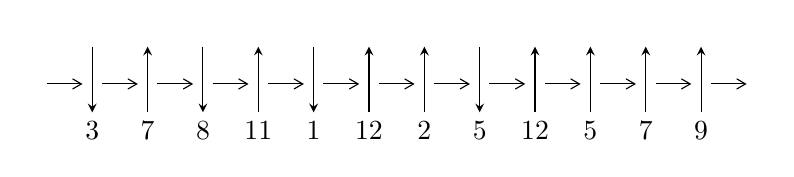
\begin{tikzpicture}[x=20pt, y=17pt]
	% nodes
	\node (C0) at (0, 0) {};
	\node (C1) at (1, 0) {};
	\node (C1U) at (1, +1) {};
	\node (C1D) at (1, -1) {3};

	\node (C2) at (2, 0) {};
	\node (C2U) at (2, +1) {};
	\node (C2D) at (2, -1) {7};

	\node (C3) at (3, 0) {};
	\node (C3U) at (3, +1) {};
	\node (C3D) at (3, -1) {8};

	\node (C4) at (4, 0) {};
	\node (C4U) at (4, +1) {};
	\node (C4D) at (4, -1) {11};

	\node (C5) at (5, 0) {};
	\node (C5U) at (5, +1) {};
	\node (C5D) at (5, -1) {1};

	\node (C6) at (6, 0) {};
	\node (C6U) at (6, +1) {};
	\node (C6D) at (6, -1) {12};

	\node (C7) at (7, 0) {};
	\node (C7U) at (7, +1) {};
	\node (C7D) at (7, -1) {2};

	\node (C8) at (8, 0) {};
	\node (C8U) at (8, +1) {};
	\node (C8D) at (8, -1) {5};

	\node (C9) at (9, 0) {};
	\node (C9U) at (9, +1) {};
	\node (C9D) at (9, -1) {12};

	\node (C10) at (10, 0) {};
	\node (C10U) at (10, +1) {};
	\node (C10D) at (10, -1) {5};

	\node (C11) at (11, 0) {};
	\node (C11U) at (11, +1) {};
	\node (C11D) at (11, -1) {7};

	\node (C12) at (12, 0) {};
	\node (C12U) at (12, +1) {};
	\node (C12D) at (12, -1) {9};
	\node (C13) at (13, 0) {};

	% arrows
	\draw[->,>={angle 60}]
	(C0) edge (C1) (C1) edge (C2) (C2) edge (C3) (C3) edge (C4) (C4) edge (C5) (C5) edge (C6) (C6) edge (C7) (C7) edge (C8) (C8) edge (C9) (C9) edge (C10) (C10) edge (C11) (C11) edge (C12) (C12) edge (C13) ;	\draw[->,>=stealth]
	(C1U) edge (C1D) (C2D) edge (C2U) (C3U) edge (C3D) (C4D) edge (C4U) (C5U) edge (C5D) (C6D) edge (C6U) (C7D) edge (C7U) (C8U) edge (C8D) (C9D) edge (C9U) (C10D) edge (C10U) (C11D) edge (C11U) (C12D) edge (C12U) ;
	\end{tikzpicture} \\
\hhline{~~} \\& 
\textbf{Solving Sequence} \\ \cline{2-2} 
 &
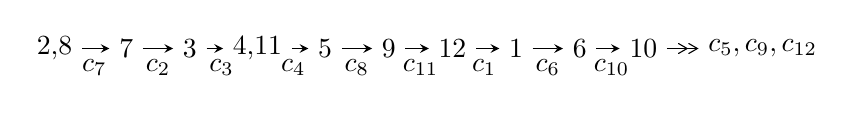
\begin{tikzpicture}[x=23pt, y=7pt]
	% node
	\node (A0) at (-1/8, 0) {2,8};
	\node (A1) at (1, 0) {7};
	\node (A2) at (2, 0) {3};
	\node (A3) at (49/16, 0) {4,11};
	\node (A4) at (33/8, 0) {5};
	\node (A5) at (41/8, 0) {9};
	\node (A6) at (49/8, 0) {12};
	\node (A7) at (57/8, 0) {1};
	\node (A8) at (65/8, 0) {6};
	\node (A9) at (73/8, 0) {10};
	\node (C1) at (1/2, -1) {$c_{7}$};
	\node (C2) at (3/2, -1) {$c_{2}$};
	\node (C3) at (5/2, -1) {$c_{3}$};
	\node (C4) at (29/8, -1) {$c_{4}$};
	\node (C5) at (37/8, -1) {$c_{8}$};
	\node (C6) at (45/8, -1) {$c_{11}$};
	\node (C7) at (53/8, -1) {$c_{1}$};
	\node (C8) at (61/8, -1) {$c_{6}$};
	\node (C9) at (69/8, -1) {$c_{10}$};
	\node (A10) at (11, 0) {$c_{5},c_{9},c_{12}$};

	% edge
	\draw[->,>=stealth]	
	(A0) edge (A1) (A1) edge (A2) (A2) edge (A3) (A3) edge (A4) (A4) edge (A5) (A5) edge (A6) (A6) edge (A7) (A7) edge (A8) (A8) edge (A9) ;
	\draw[->>,>={angle 60}]	
	(A9) edge (A10);
\end{tikzpicture} \\ 

\end{tabular} \\

\footnotetext{
The image of knot diagram is generated by the software ``\textbf{Draw programme}" developed by Andrew Bartholomew(\url{http://www.layer8.co.uk/maths/draw/index.htm\#Running-draw}), where we modified some parts for our purpose(\url{https://github.com/CATsTAILs/LinksPainter}).
}\phantom \\ \newline 
\centering \textbf{Ideals for irreducible components\footnotemark of $X_{\text{par}}$} 
 
\begin{align*}
I^u_{1}&=\langle 
5 u^{20}+56 u^{19}+\cdots+4 b-116,\;9 u^{20}+75 u^{19}+\cdots+16 a+72,\;u^{21}+11 u^{20}+\cdots-80 u-16\rangle \\
I^u_{2}&=\langle 
- u^{16}+u^{15}+\cdots+b+5,\;-3 u^{16}-9 u^{15}+\cdots+2 a-4,\;u^{17}+u^{16}+\cdots+2 u+2\rangle \\
\\
\end{align*}
\raggedright * 2 irreducible components of $\dim_{\mathbb{C}}=0$, with total 38 representations.\\
\footnotetext{All coefficients of polynomials are rational numbers. But the coefficients are sometimes approximated in decimal forms when there is not enough margin.}
\newpage
\renewcommand{\arraystretch}{1}
\centering \section*{I. $I^u_{1}= \langle 5 u^{20}+56 u^{19}+\cdots+4 b-116,\;9 u^{20}+75 u^{19}+\cdots+16 a+72,\;u^{21}+11 u^{20}+\cdots-80 u-16 \rangle$}
\flushleft \textbf{(i) Arc colorings}\\
\begin{tabular}{m{7pt} m{180pt} m{7pt} m{180pt} }
\flushright $a_{2}=$&$\begin{pmatrix}0\\u\end{pmatrix}$ \\
\flushright $a_{8}=$&$\begin{pmatrix}1\\0\end{pmatrix}$ \\
\flushright $a_{7}=$&$\begin{pmatrix}1\\u^2\end{pmatrix}$ \\
\flushright $a_{3}=$&$\begin{pmatrix}u\\u^3+u\end{pmatrix}$ \\
\flushright $a_{4}=$&$\begin{pmatrix}- u^3\\u^3+u\end{pmatrix}$ \\
\flushright $a_{11}=$&$\begin{pmatrix}-0.562500 u^{20}-4.68750 u^{19}+\cdots-16.7500 u-4.50000\\-\frac{5}{4} u^{20}-14 u^{19}+\cdots+\frac{241}{2} u+29\end{pmatrix}$ \\
\flushright $a_{5}=$&$\begin{pmatrix}\frac{3}{16} u^{20}+\frac{31}{16} u^{19}+\cdots-\frac{85}{8} u^2-\frac{7}{2} u\\-\frac{5}{8} u^{20}-\frac{49}{8} u^{19}+\cdots+29 u+7\end{pmatrix}$ \\
\flushright $a_{9}=$&$\begin{pmatrix}\frac{3}{8} u^{20}+3 u^{19}+\cdots+\frac{159}{4} u+\frac{23}{2}\\\frac{11}{8} u^{20}+\frac{121}{8} u^{19}+\cdots-\frac{275}{2} u-34\end{pmatrix}$ \\
\flushright $a_{12}=$&$\begin{pmatrix}-0.562500 u^{20}-4.43750 u^{19}+\cdots-7.25000 u+0.500000\\-\frac{7}{4} u^{20}-\frac{39}{2} u^{19}+\cdots+\frac{281}{2} u+33\end{pmatrix}$ \\
\flushright $a_{1}=$&$\begin{pmatrix}u^3\\u^5+u^3+u\end{pmatrix}$ \\
\flushright $a_{6}=$&$\begin{pmatrix}\frac{3}{16} u^{20}+\frac{31}{16} u^{19}+\cdots-\frac{63}{2} u-8\\\frac{9}{8} u^{20}+\frac{85}{8} u^{19}+\cdots-42 u-11\end{pmatrix}$ \\
\flushright $a_{10}=$&$\begin{pmatrix}-\frac{11}{16} u^{20}-\frac{85}{16} u^{19}+\cdots-\frac{213}{4} u-14\\-\frac{5}{2} u^{20}-27 u^{19}+\cdots+225 u+55\end{pmatrix}$\\&\end{tabular}
\flushleft \textbf{(ii) Obstruction class $= -1$}\\~\\
\flushleft \textbf{(iii) Cusp Shapes $= \frac{21}{2} u^{20}+\frac{225}{2} u^{19}+\frac{1289}{2} u^{18}+2524 u^{17}+\frac{14905}{2} u^{16}+\frac{34975}{2} u^{15}+\frac{67375}{2} u^{14}+54537 u^{13}+\frac{151085}{2} u^{12}+\frac{181727}{2} u^{11}+\frac{191943}{2} u^{10}+\frac{179037}{2} u^9+73543 u^8+52381 u^7+31237 u^6+\frac{28777}{2} u^5+3949 u^4-589 u^3-1353 u^2-726 u-166$}\\~\\
\newpage\renewcommand{\arraystretch}{1}
\flushleft \textbf{(iv) u-Polynomials at the component}\newline \\
\begin{tabular}{m{50pt}|m{274pt}}
Crossings & \hspace{64pt}u-Polynomials at each crossing \\
\hline $$\begin{aligned}c_{1}\end{aligned}$$&$\begin{aligned}
&u^{21}+9 u^{20}+\cdots+896 u-256
\end{aligned}$\\
\hline $$\begin{aligned}c_{2},c_{7}\end{aligned}$$&$\begin{aligned}
&u^{21}+11 u^{20}+\cdots-80 u-16
\end{aligned}$\\
\hline $$\begin{aligned}c_{3}\end{aligned}$$&$\begin{aligned}
&u^{21}-11 u^{20}+\cdots-8656 u-2512
\end{aligned}$\\
\hline $$\begin{aligned}c_{4},c_{6},c_{10}\\c_{11}\end{aligned}$$&$\begin{aligned}
&u^{21}+27 u^{19}+\cdots+u-1
\end{aligned}$\\
\hline $$\begin{aligned}c_{5},c_{8}\end{aligned}$$&$\begin{aligned}
&u^{21}+2 u^{20}+\cdots+28 u^2-1
\end{aligned}$\\
\hline $$\begin{aligned}c_{9},c_{12}\end{aligned}$$&$\begin{aligned}
&u^{21}+4 u^{20}+\cdots-5 u-1
\end{aligned}$\\
\hline
\end{tabular}\\~\\
\newpage\renewcommand{\arraystretch}{1}
\flushleft \textbf{(v) Riley Polynomials at the component}\newline \\
\begin{tabular}{m{50pt}|m{274pt}}
Crossings & \hspace{64pt}Riley Polynomials at each crossing \\
\hline $$\begin{aligned}c_{1}\end{aligned}$$&$\begin{aligned}
&y^{21}+5 y^{20}+\cdots+2367488 y-65536
\end{aligned}$\\
\hline $$\begin{aligned}c_{2},c_{7}\end{aligned}$$&$\begin{aligned}
&y^{21}+9 y^{20}+\cdots+896 y-256
\end{aligned}$\\
\hline $$\begin{aligned}c_{3}\end{aligned}$$&$\begin{aligned}
&y^{21}-107 y^{20}+\cdots-395058816 y-6310144
\end{aligned}$\\
\hline $$\begin{aligned}c_{4},c_{6},c_{10}\\c_{11}\end{aligned}$$&$\begin{aligned}
&y^{21}+54 y^{20}+\cdots-9 y-1
\end{aligned}$\\
\hline $$\begin{aligned}c_{5},c_{8}\end{aligned}$$&$\begin{aligned}
&y^{21}-46 y^{20}+\cdots+56 y-1
\end{aligned}$\\
\hline $$\begin{aligned}c_{9},c_{12}\end{aligned}$$&$\begin{aligned}
&y^{21}+2 y^{20}+\cdots- y-1
\end{aligned}$\\
\hline
\end{tabular}\\~\\
\newpage\flushleft \textbf{(vi) Complex Volumes and Cusp Shapes}
$$\begin{array}{c|c|c}  
\text{Solutions to }I^u_{1}& \I (\text{vol} + \sqrt{-1}CS) & \text{Cusp shape}\\
 \hline 
\begin{aligned}
u &= \phantom{-}0.472469 + 0.828155 I \\
a &= -0.488123 - 0.166277 I \\
b &= \phantom{-}0.188036 + 0.222130 I\end{aligned}
 & \phantom{-}0.20225 + 1.98003 I & \phantom{-}2.28798 - 3.26174 I \\ \hline\begin{aligned}
u &= \phantom{-}0.472469 - 0.828155 I \\
a &= -0.488123 + 0.166277 I \\
b &= \phantom{-}0.188036 - 0.222130 I\end{aligned}
 & \phantom{-}0.20225 - 1.98003 I & \phantom{-}2.28798 + 3.26174 I \\ \hline\begin{aligned}
u &= -0.771804 + 0.719603 I \\
a &= -1.319550 - 0.250548 I \\
b &= \phantom{-}0.47482 + 1.81639 I\end{aligned}
 & \phantom{-}3.69054 + 0.94413 I & \phantom{-}3.84004 + 4.58061 I \\ \hline\begin{aligned}
u &= -0.771804 - 0.719603 I \\
a &= -1.319550 + 0.250548 I \\
b &= \phantom{-}0.47482 - 1.81639 I\end{aligned}
 & \phantom{-}3.69054 - 0.94413 I & \phantom{-}3.84004 - 4.58061 I \\ \hline\begin{aligned}
u &= \phantom{-}0.036593 + 0.936717 I \\
a &= \phantom{-}0.078038 - 0.908614 I \\
b &= -0.472625 + 0.388644 I\end{aligned}
 & -1.84690 + 1.45685 I & -2.25321 - 5.17450 I \\ \hline\begin{aligned}
u &= \phantom{-}0.036593 - 0.936717 I \\
a &= \phantom{-}0.078038 + 0.908614 I \\
b &= -0.472625 - 0.388644 I\end{aligned}
 & -1.84690 - 1.45685 I & -2.25321 + 5.17450 I \\ \hline\begin{aligned}
u &= -0.710005 + 0.988627 I \\
a &= \phantom{-}1.54173 + 0.94297 I \\
b &= -0.24228 - 2.12126 I\end{aligned}
 & \phantom{-}2.87016 - 6.56510 I & -1.92301 + 3.76598 I \\ \hline\begin{aligned}
u &= -0.710005 - 0.988627 I \\
a &= \phantom{-}1.54173 - 0.94297 I \\
b &= -0.24228 + 2.12126 I\end{aligned}
 & \phantom{-}2.87016 + 6.56510 I & -1.92301 - 3.76598 I \\ \hline\begin{aligned}
u &= -0.769484 + 0.051011 I \\
a &= -0.141173 + 0.103619 I \\
b &= -0.347832 + 0.454102 I\end{aligned}
 & -2.61653 + 1.28499 I & \phantom{-}0.15587 - 3.07961 I \\ \hline\begin{aligned}
u &= -0.769484 - 0.051011 I \\
a &= -0.141173 - 0.103619 I \\
b &= -0.347832 - 0.454102 I\end{aligned}
 & -2.61653 - 1.28499 I & \phantom{-}0.15587 + 3.07961 I\\
 \hline 
 \end{array}$$\newpage$$\begin{array}{c|c|c}  
\text{Solutions to }I^u_{1}& \I (\text{vol} + \sqrt{-1}CS) & \text{Cusp shape}\\
 \hline 
\begin{aligned}
u &= -0.435565 + 1.195780 I \\
a &= -0.004901 - 0.689508 I \\
b &= -0.468235 + 0.470276 I\end{aligned}
 & -6.21856 - 2.94897 I & -0.504582 + 0.049416 I \\ \hline\begin{aligned}
u &= -0.435565 - 1.195780 I \\
a &= -0.004901 + 0.689508 I \\
b &= -0.468235 - 0.470276 I\end{aligned}
 & -6.21856 + 2.94897 I & -0.504582 - 0.049416 I \\ \hline\begin{aligned}
u &= -0.472104 + 1.199130 I \\
a &= \phantom{-}0.644752 + 0.145048 I \\
b &= -0.345148 - 0.550837 I\end{aligned}
 & -5.96069 - 5.81849 I & -5.01229 + 8.57270 I \\ \hline\begin{aligned}
u &= -0.472104 - 1.199130 I \\
a &= \phantom{-}0.644752 - 0.145048 I \\
b &= -0.345148 + 0.550837 I\end{aligned}
 & -5.96069 + 5.81849 I & -5.01229 - 8.57270 I \\ \hline\begin{aligned}
u &= -1.49061 + 0.03728 I \\
a &= \phantom{-}0.034735 + 0.714146 I \\
b &= \phantom{-}0.00483 - 2.16677 I\end{aligned}
 & -15.8145 - 3.8268 I & \phantom{-}1.96641 + 1.96096 I \\ \hline\begin{aligned}
u &= -1.49061 - 0.03728 I \\
a &= \phantom{-}0.034735 - 0.714146 I \\
b &= \phantom{-}0.00483 + 2.16677 I\end{aligned}
 & -15.8145 + 3.8268 I & \phantom{-}1.96641 - 1.96096 I \\ \hline\begin{aligned}
u &= \phantom{-}0.423148\phantom{ +0.000000I} \\
a &= -1.20478\phantom{ +0.000000I} \\
b &= \phantom{-}0.358221\phantom{ +0.000000I}\end{aligned}
 & \phantom{-}0.913214\phantom{ +0.000000I} & \phantom{-}11.0410\phantom{ +0.000000I} \\ \hline\begin{aligned}
u &= -0.76209 + 1.50016 I \\
a &= \phantom{-}1.21983 + 1.44613 I \\
b &= -0.15370 - 2.09019 I\end{aligned}
 & \phantom{-}19.0348 - 11.6307 I & \phantom{-0.000000 -}0. + 4.72402 I \\ \hline\begin{aligned}
u &= -0.76209 - 1.50016 I \\
a &= \phantom{-}1.21983 - 1.44613 I \\
b &= -0.15370 + 2.09019 I\end{aligned}
 & \phantom{-}19.0348 + 11.6307 I & \phantom{-0.000000 } 0. - 4.72402 I \\ \hline\begin{aligned}
u &= -0.80898 + 1.48155 I \\
a &= -1.21294 - 1.39486 I \\
b &= \phantom{-}0.18302 + 2.08076 I\end{aligned}
 & \phantom{-}19.3623 - 4.1247 I & \phantom{-0.000000 } 0\\
 \hline 
 \end{array}$$\newpage$$\begin{array}{c|c|c}  
\text{Solutions to }I^u_{1}& \I (\text{vol} + \sqrt{-1}CS) & \text{Cusp shape}\\
 \hline 
\begin{aligned}
u &= -0.80898 - 1.48155 I \\
a &= -1.21294 + 1.39486 I \\
b &= \phantom{-}0.18302 - 2.08076 I\end{aligned}
 & \phantom{-}19.3623 + 4.1247 I & \phantom{-0.000000 } 0\\
 \hline 
 \end{array}$$\newpage\newpage\renewcommand{\arraystretch}{1}
\centering \section*{II. $I^u_{2}= \langle - u^{16}+u^{15}+\cdots+b+5,\;-3 u^{16}-9 u^{15}+\cdots+2 a-4,\;u^{17}+u^{16}+\cdots+2 u+2 \rangle$}
\flushleft \textbf{(i) Arc colorings}\\
\begin{tabular}{m{7pt} m{180pt} m{7pt} m{180pt} }
\flushright $a_{2}=$&$\begin{pmatrix}0\\u\end{pmatrix}$ \\
\flushright $a_{8}=$&$\begin{pmatrix}1\\0\end{pmatrix}$ \\
\flushright $a_{7}=$&$\begin{pmatrix}1\\u^2\end{pmatrix}$ \\
\flushright $a_{3}=$&$\begin{pmatrix}u\\u^3+u\end{pmatrix}$ \\
\flushright $a_{4}=$&$\begin{pmatrix}- u^3\\u^3+u\end{pmatrix}$ \\
\flushright $a_{11}=$&$\begin{pmatrix}\frac{3}{2} u^{16}+\frac{9}{2} u^{15}+\cdots+\frac{19}{2} u+2\\u^{16}- u^{15}+\cdots-8 u-5\end{pmatrix}$ \\
\flushright $a_{5}=$&$\begin{pmatrix}-\frac{1}{2} u^{16}-\frac{3}{2} u^{15}+\cdots+\frac{3}{2} u-1\\u^{15}+u^{14}+\cdots+2 u+1\end{pmatrix}$ \\
\flushright $a_{9}=$&$\begin{pmatrix}\frac{5}{2} u^{16}+\frac{11}{2} u^{15}+\cdots+\frac{21}{2} u+8\\u^{16}- u^{15}+\cdots-4 u-5\end{pmatrix}$ \\
\flushright $a_{12}=$&$\begin{pmatrix}\frac{5}{2} u^{16}+\frac{13}{2} u^{15}+\cdots+\frac{21}{2} u+3\\-3 u^{15}-5 u^{14}+\cdots-12 u-7\end{pmatrix}$ \\
\flushright $a_{1}=$&$\begin{pmatrix}u^3\\u^5+u^3+u\end{pmatrix}$ \\
\flushright $a_{6}=$&$\begin{pmatrix}-\frac{3}{2} u^{16}-\frac{5}{2} u^{15}+\cdots-\frac{1}{2} u-1\\u^{16}+2 u^{15}+\cdots+3 u+1\end{pmatrix}$ \\
\flushright $a_{10}=$&$\begin{pmatrix}5 u^{16}+9 u^{15}+\cdots+20 u+6\\u^{16}-3 u^{15}+\cdots-13 u-10\end{pmatrix}$\\&\end{tabular}
\flushleft \textbf{(ii) Obstruction class $= 1$}\\~\\
\flushleft \textbf{(iii) Cusp Shapes $= u^{16}-2 u^{15}-3 u^{14}-13 u^{13}-16 u^{12}-34 u^{11}-48 u^{10}-74 u^9-85 u^8-100 u^7-105 u^6-105 u^5-96 u^4-75 u^3-56 u^2-30 u-16$}\\~\\
\newpage\renewcommand{\arraystretch}{1}
\flushleft \textbf{(iv) u-Polynomials at the component}\newline \\
\begin{tabular}{m{50pt}|m{274pt}}
Crossings & \hspace{64pt}u-Polynomials at each crossing \\
\hline $$\begin{aligned}c_{1}\end{aligned}$$&$\begin{aligned}
&u^{17}-9 u^{16}+\cdots-32 u+4
\end{aligned}$\\
\hline $$\begin{aligned}c_{2}\end{aligned}$$&$\begin{aligned}
&u^{17}- u^{16}+\cdots+2 u-2
\end{aligned}$\\
\hline $$\begin{aligned}c_{3}\end{aligned}$$&$\begin{aligned}
&u^{17}+u^{16}+\cdots+6 u-2
\end{aligned}$\\
\hline $$\begin{aligned}c_{4},c_{11}\end{aligned}$$&$\begin{aligned}
&u^{17}+u^{16}+\cdots- u-1
\end{aligned}$\\
\hline $$\begin{aligned}c_{5},c_{8}\end{aligned}$$&$\begin{aligned}
&u^{17}- u^{16}+\cdots+2 u+1
\end{aligned}$\\
\hline $$\begin{aligned}c_{6},c_{10}\end{aligned}$$&$\begin{aligned}
&u^{17}- u^{16}+\cdots- u+1
\end{aligned}$\\
\hline $$\begin{aligned}c_{7}\end{aligned}$$&$\begin{aligned}
&u^{17}+u^{16}+\cdots+2 u+2
\end{aligned}$\\
\hline $$\begin{aligned}c_{9}\end{aligned}$$&$\begin{aligned}
&u^{17}+7 u^{16}+\cdots+5 u+1
\end{aligned}$\\
\hline $$\begin{aligned}c_{12}\end{aligned}$$&$\begin{aligned}
&u^{17}-7 u^{16}+\cdots+5 u-1
\end{aligned}$\\
\hline
\end{tabular}\\~\\
\newpage\renewcommand{\arraystretch}{1}
\flushleft \textbf{(v) Riley Polynomials at the component}\newline \\
\begin{tabular}{m{50pt}|m{274pt}}
Crossings & \hspace{64pt}Riley Polynomials at each crossing \\
\hline $$\begin{aligned}c_{1}\end{aligned}$$&$\begin{aligned}
&y^{17}+5 y^{16}+\cdots-8 y-16
\end{aligned}$\\
\hline $$\begin{aligned}c_{2},c_{7}\end{aligned}$$&$\begin{aligned}
&y^{17}+9 y^{16}+\cdots-32 y-4
\end{aligned}$\\
\hline $$\begin{aligned}c_{3}\end{aligned}$$&$\begin{aligned}
&y^{17}+y^{16}+\cdots-24 y-4
\end{aligned}$\\
\hline $$\begin{aligned}c_{4},c_{6},c_{10}\\c_{11}\end{aligned}$$&$\begin{aligned}
&y^{17}+5 y^{16}+\cdots+9 y-1
\end{aligned}$\\
\hline $$\begin{aligned}c_{5},c_{8}\end{aligned}$$&$\begin{aligned}
&y^{17}-3 y^{16}+\cdots-6 y-1
\end{aligned}$\\
\hline $$\begin{aligned}c_{9},c_{12}\end{aligned}$$&$\begin{aligned}
&y^{17}+y^{16}+\cdots+y-1
\end{aligned}$\\
\hline
\end{tabular}\\~\\
\newpage\flushleft \textbf{(vi) Complex Volumes and Cusp Shapes}
$$\begin{array}{c|c|c}  
\text{Solutions to }I^u_{2}& \I (\text{vol} + \sqrt{-1}CS) & \text{Cusp shape}\\
 \hline 
\begin{aligned}
u &= \phantom{-}0.281134 + 0.946456 I \\
a &= \phantom{-}1.24113 - 1.45623 I \\
b &= \phantom{-}0.36623 + 1.54673 I\end{aligned}
 & \phantom{-}0.52851 - 1.83462 I & \phantom{-}0.29796 + 3.58847 I \\ \hline\begin{aligned}
u &= \phantom{-}0.281134 - 0.946456 I \\
a &= \phantom{-}1.24113 + 1.45623 I \\
b &= \phantom{-}0.36623 - 1.54673 I\end{aligned}
 & \phantom{-}0.52851 + 1.83462 I & \phantom{-}0.29796 - 3.58847 I \\ \hline\begin{aligned}
u &= -0.969290\phantom{ +0.000000I} \\
a &= \phantom{-}0.776451\phantom{ +0.000000I} \\
b &= -0.382171\phantom{ +0.000000I}\end{aligned}
 & -1.53916\phantom{ +0.000000I} & \phantom{-}3.39910\phantom{ +0.000000I} \\ \hline\begin{aligned}
u &= \phantom{-}0.728050 + 0.766886 I \\
a &= \phantom{-}1.70484 - 0.42800 I \\
b &= -0.50880 + 2.22693 I\end{aligned}
 & \phantom{-}3.93432 - 1.40561 I & \phantom{-}11.9334 + 8.1612 I \\ \hline\begin{aligned}
u &= \phantom{-}0.728050 - 0.766886 I \\
a &= \phantom{-}1.70484 + 0.42800 I \\
b &= -0.50880 - 2.22693 I\end{aligned}
 & \phantom{-}3.93432 + 1.40561 I & \phantom{-}11.9334 - 8.1612 I \\ \hline\begin{aligned}
u &= \phantom{-}0.224277 + 0.858763 I \\
a &= -1.56206 + 0.82631 I \\
b &= \phantom{-}0.127397 - 1.349340 I\end{aligned}
 & \phantom{-}0.93314 + 4.06440 I & \phantom{-}0.37552 - 3.75729 I \\ \hline\begin{aligned}
u &= \phantom{-}0.224277 - 0.858763 I \\
a &= -1.56206 - 0.82631 I \\
b &= \phantom{-}0.127397 + 1.349340 I\end{aligned}
 & \phantom{-}0.93314 - 4.06440 I & \phantom{-}0.37552 + 3.75729 I \\ \hline\begin{aligned}
u &= -0.737443 + 0.842981 I \\
a &= \phantom{-}1.105660 - 0.250731 I \\
b &= -0.533874 + 0.383844 I\end{aligned}
 & -3.11346 - 2.81675 I & \phantom{-}2.33737 + 2.85701 I \\ \hline\begin{aligned}
u &= -0.737443 - 0.842981 I \\
a &= \phantom{-}1.105660 + 0.250731 I \\
b &= -0.533874 - 0.383844 I\end{aligned}
 & -3.11346 + 2.81675 I & \phantom{-}2.33737 - 2.85701 I \\ \hline\begin{aligned}
u &= -0.382757 + 1.099770 I \\
a &= -0.682974 - 0.515143 I \\
b &= \phantom{-}0.561927 + 0.046321 I\end{aligned}
 & -7.10806 - 3.64002 I & -7.66149 + 4.40489 I\\
 \hline 
 \end{array}$$\newpage$$\begin{array}{c|c|c}  
\text{Solutions to }I^u_{2}& \I (\text{vol} + \sqrt{-1}CS) & \text{Cusp shape}\\
 \hline 
\begin{aligned}
u &= -0.382757 - 1.099770 I \\
a &= -0.682974 + 0.515143 I \\
b &= \phantom{-}0.561927 - 0.046321 I\end{aligned}
 & -7.10806 + 3.64002 I & -7.66149 - 4.40489 I \\ \hline\begin{aligned}
u &= \phantom{-}0.676951 + 0.964759 I \\
a &= -1.78717 + 1.20472 I \\
b &= \phantom{-}0.10658 - 2.49443 I\end{aligned}
 & \phantom{-}3.30875 + 6.79114 I & \phantom{-}13.3760 - 11.7173 I \\ \hline\begin{aligned}
u &= \phantom{-}0.676951 - 0.964759 I \\
a &= -1.78717 - 1.20472 I \\
b &= \phantom{-}0.10658 + 2.49443 I\end{aligned}
 & \phantom{-}3.30875 - 6.79114 I & \phantom{-}13.3760 + 11.7173 I \\ \hline\begin{aligned}
u &= -0.306582 + 0.677700 I \\
a &= -1.79619 + 0.12408 I \\
b &= \phantom{-}0.674089 - 0.611126 I\end{aligned}
 & -5.45769 + 0.67304 I & -4.27931 - 3.12764 I \\ \hline\begin{aligned}
u &= -0.306582 - 0.677700 I \\
a &= -1.79619 - 0.12408 I \\
b &= \phantom{-}0.674089 + 0.611126 I\end{aligned}
 & -5.45769 - 0.67304 I & -4.27931 + 3.12764 I \\ \hline\begin{aligned}
u &= -0.498985 + 1.260640 I \\
a &= \phantom{-}0.388541 - 0.408565 I \\
b &= -0.102456 + 0.376600 I\end{aligned}
 & -5.41541 - 5.16567 I & \phantom{-}1.42099 + 1.44225 I \\ \hline\begin{aligned}
u &= -0.498985 - 1.260640 I \\
a &= \phantom{-}0.388541 + 0.408565 I \\
b &= -0.102456 - 0.376600 I\end{aligned}
 & -5.41541 + 5.16567 I & \phantom{-}1.42099 - 1.44225 I\\
 \hline 
 \end{array}$$\newpage
\newpage\renewcommand{\arraystretch}{1}
\centering \section*{ III. u-Polynomials}
\begin{tabular}{m{50pt}|m{274pt}}
Crossings & \hspace{64pt}u-Polynomials at each crossing \\
\hline $$\begin{aligned}c_{1}\end{aligned}$$&$\begin{aligned}
&(u^{17}-9 u^{16}+\cdots-32 u+4)(u^{21}+9 u^{20}+\cdots+896 u-256)
\end{aligned}$\\
\hline $$\begin{aligned}c_{2}\end{aligned}$$&$\begin{aligned}
&(u^{17}- u^{16}+\cdots+2 u-2)(u^{21}+11 u^{20}+\cdots-80 u-16)
\end{aligned}$\\
\hline $$\begin{aligned}c_{3}\end{aligned}$$&$\begin{aligned}
&(u^{17}+u^{16}+\cdots+6 u-2)(u^{21}-11 u^{20}+\cdots-8656 u-2512)
\end{aligned}$\\
\hline $$\begin{aligned}c_{4},c_{11}\end{aligned}$$&$\begin{aligned}
&(u^{17}+u^{16}+\cdots- u-1)(u^{21}+27 u^{19}+\cdots+u-1)
\end{aligned}$\\
\hline $$\begin{aligned}c_{5},c_{8}\end{aligned}$$&$\begin{aligned}
&(u^{17}- u^{16}+\cdots+2 u+1)(u^{21}+2 u^{20}+\cdots+28 u^2-1)
\end{aligned}$\\
\hline $$\begin{aligned}c_{6},c_{10}\end{aligned}$$&$\begin{aligned}
&(u^{17}- u^{16}+\cdots- u+1)(u^{21}+27 u^{19}+\cdots+u-1)
\end{aligned}$\\
\hline $$\begin{aligned}c_{7}\end{aligned}$$&$\begin{aligned}
&(u^{17}+u^{16}+\cdots+2 u+2)(u^{21}+11 u^{20}+\cdots-80 u-16)
\end{aligned}$\\
\hline $$\begin{aligned}c_{9}\end{aligned}$$&$\begin{aligned}
&(u^{17}+7 u^{16}+\cdots+5 u+1)(u^{21}+4 u^{20}+\cdots-5 u-1)
\end{aligned}$\\
\hline $$\begin{aligned}c_{12}\end{aligned}$$&$\begin{aligned}
&(u^{17}-7 u^{16}+\cdots+5 u-1)(u^{21}+4 u^{20}+\cdots-5 u-1)
\end{aligned}$\\
\hline
\end{tabular}\newpage\renewcommand{\arraystretch}{1}
\centering \section*{ IV. Riley Polynomials}
\begin{tabular}{m{50pt}|m{274pt}}
Crossings & \hspace{64pt}Riley Polynomials at each crossing \\
\hline $$\begin{aligned}c_{1}\end{aligned}$$&$\begin{aligned}
&(y^{17}+5 y^{16}+\cdots-8 y-16)(y^{21}+5 y^{20}+\cdots+2367488 y-65536)
\end{aligned}$\\
\hline $$\begin{aligned}c_{2},c_{7}\end{aligned}$$&$\begin{aligned}
&(y^{17}+9 y^{16}+\cdots-32 y-4)(y^{21}+9 y^{20}+\cdots+896 y-256)
\end{aligned}$\\
\hline $$\begin{aligned}c_{3}\end{aligned}$$&$\begin{aligned}
&(y^{17}+y^{16}+\cdots-24 y-4)\\
&\cdot(y^{21}-107 y^{20}+\cdots-395058816 y-6310144)
\end{aligned}$\\
\hline $$\begin{aligned}c_{4},c_{6},c_{10}\\c_{11}\end{aligned}$$&$\begin{aligned}
&(y^{17}+5 y^{16}+\cdots+9 y-1)(y^{21}+54 y^{20}+\cdots-9 y-1)
\end{aligned}$\\
\hline $$\begin{aligned}c_{5},c_{8}\end{aligned}$$&$\begin{aligned}
&(y^{17}-3 y^{16}+\cdots-6 y-1)(y^{21}-46 y^{20}+\cdots+56 y-1)
\end{aligned}$\\
\hline $$\begin{aligned}c_{9},c_{12}\end{aligned}$$&$\begin{aligned}
&(y^{17}+y^{16}+\cdots+y-1)(y^{21}+2 y^{20}+\cdots- y-1)
\end{aligned}$\\
\hline
\end{tabular}
\vskip 2pc
\end{document}